\chapter{Project Design}

\section{Software Requirement Specification}

\subsection{Hardware Requirements}
\\
\begin{itemize}
\item {2.4GHz Celeron Processor}
\item {256MB Memory}
\item {10GB Disk Space}
\end{itemize}

\subsection{Software Requirements}
\\
\begin{itemize}
\item {[Operating System]: Linux Based Operating System}
\item {[Build-essential]: Build-essential is required to build Debian packages, starting with dpkg (\textgreater= 1.14.18)}
\item {[Necessary packages for building GCC]:\\ \url{http://gcc.gnu.org/install/prerequisites.html}}
\end{itemize}

\subsection{Technologies Used}
\\
\begin{itemize}
\item C, lex, yacc.
\end{itemize}
\newpage
\section{U.M.L. Diagrams}

\subsection{Use Case}
\begin{figure}[H]
\centering
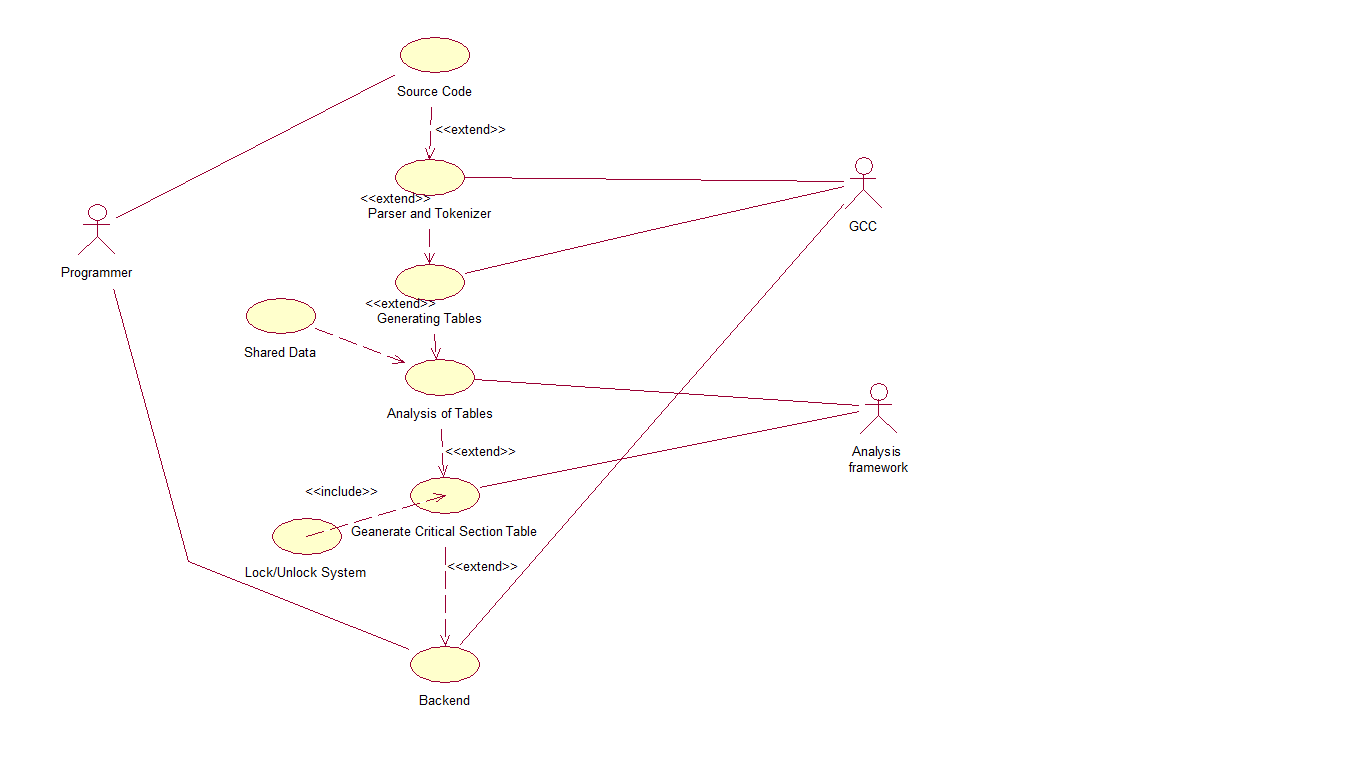
\includegraphics[scale=0.6]{usecase.png}
\caption{Use case diagram}
\label{<<Label>>}
\end{figure}
\paragraph{}
From use case point of view our system contains one actor as user or programmer, in which programmer has to specify a C source code (Source code should be error free and Multithreaded for better results).
And on the other hand GCC does the parsing and tokenization with the help of patterns and grammar that we have written, Analysis framework does the detection of critical sections in a source code provided by the Programmer as a input.


\subsection{State Chart}
\begin{figure}[H]
\centering
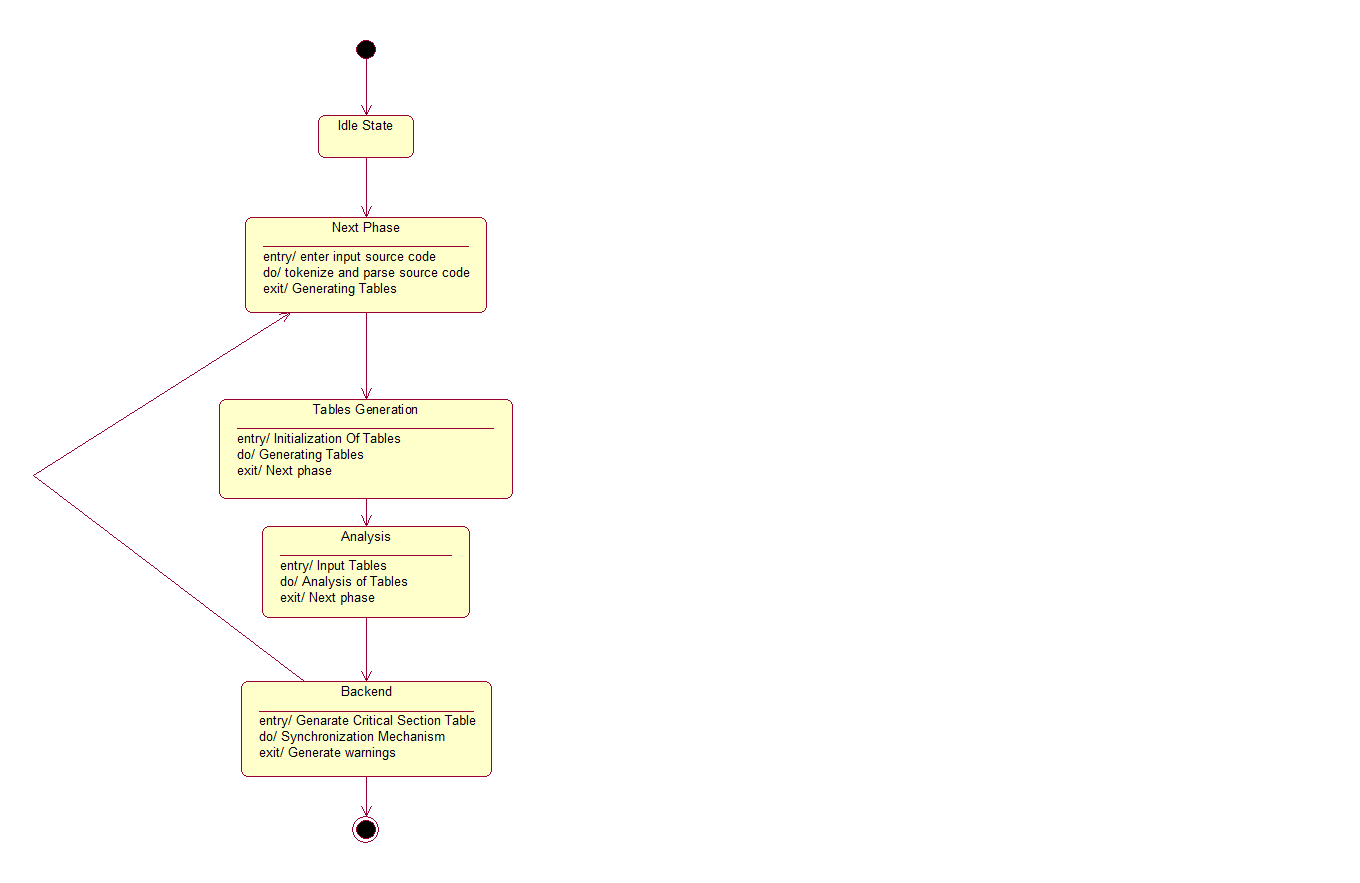
\includegraphics[scale=0.7]{statechart.png}
\caption{State chart diagram}
\label{<<Label>>}
\end{figure}
\paragraph{}
Control Flow of the Critical Section Detection System.
Above figure shows the state transisions of our system, this shows that how actually the system is going to transfer from eact step to next step after providing certain input. There are certain steps in each state. Flow of the Critical Section Detection System.

\subsection{Sequence Diagram}
\begin{figure}[H]
\centering
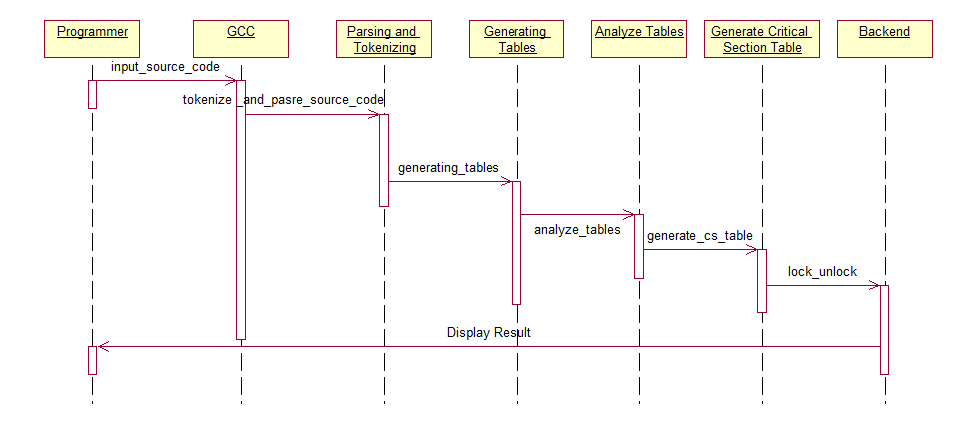
\includegraphics[scale=0.5]{sequence.png}
\caption{Sequence Diagram}
\label{<<Label>>}
\end{figure}
\paragraph{}
Shows the sequences of operations from starting to last one. A sequence diagram shows object interactions arranged in time sequence. It depicts the objects and classes involved in the scenario i.e Programmer, GCC, Analysis Framework etc. and the sequence of messages exchanged between the objects needed to carry out the functionality of the scenario. Scenario could be whole sequence of operations till the end result.  

\subsection{Collaboration Diagram}
\begin{figure}[H]
\centering
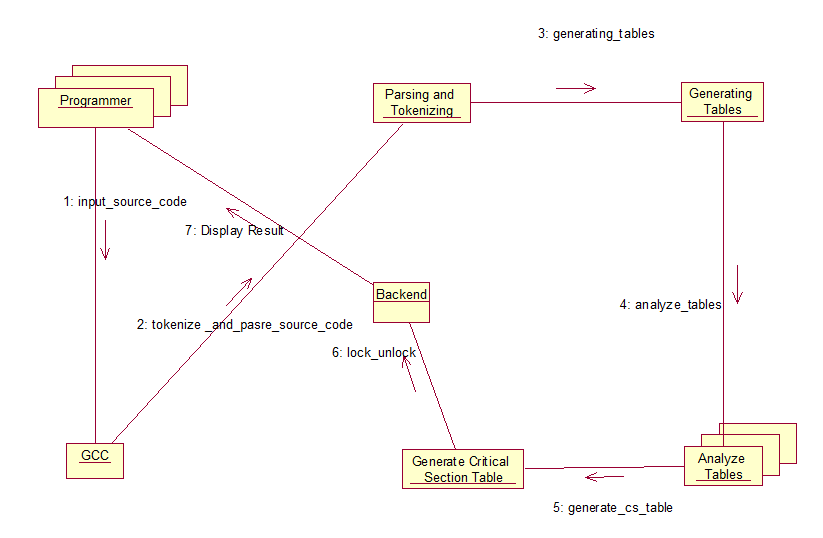
\includegraphics[scale=0.6]{collaboration.png}
\caption{Collaboration Diagram}
\label{<<Label>>}
\end{figure}
\paragraph{}
From Collaboarative perspective of our system, it covers the same scenario as shown in Sequence diagram.Indeed the collaborative view of the system is generated by using sequence diagram. 

\subsection{Activity Diagram}
\begin{figure}[H]
\centering
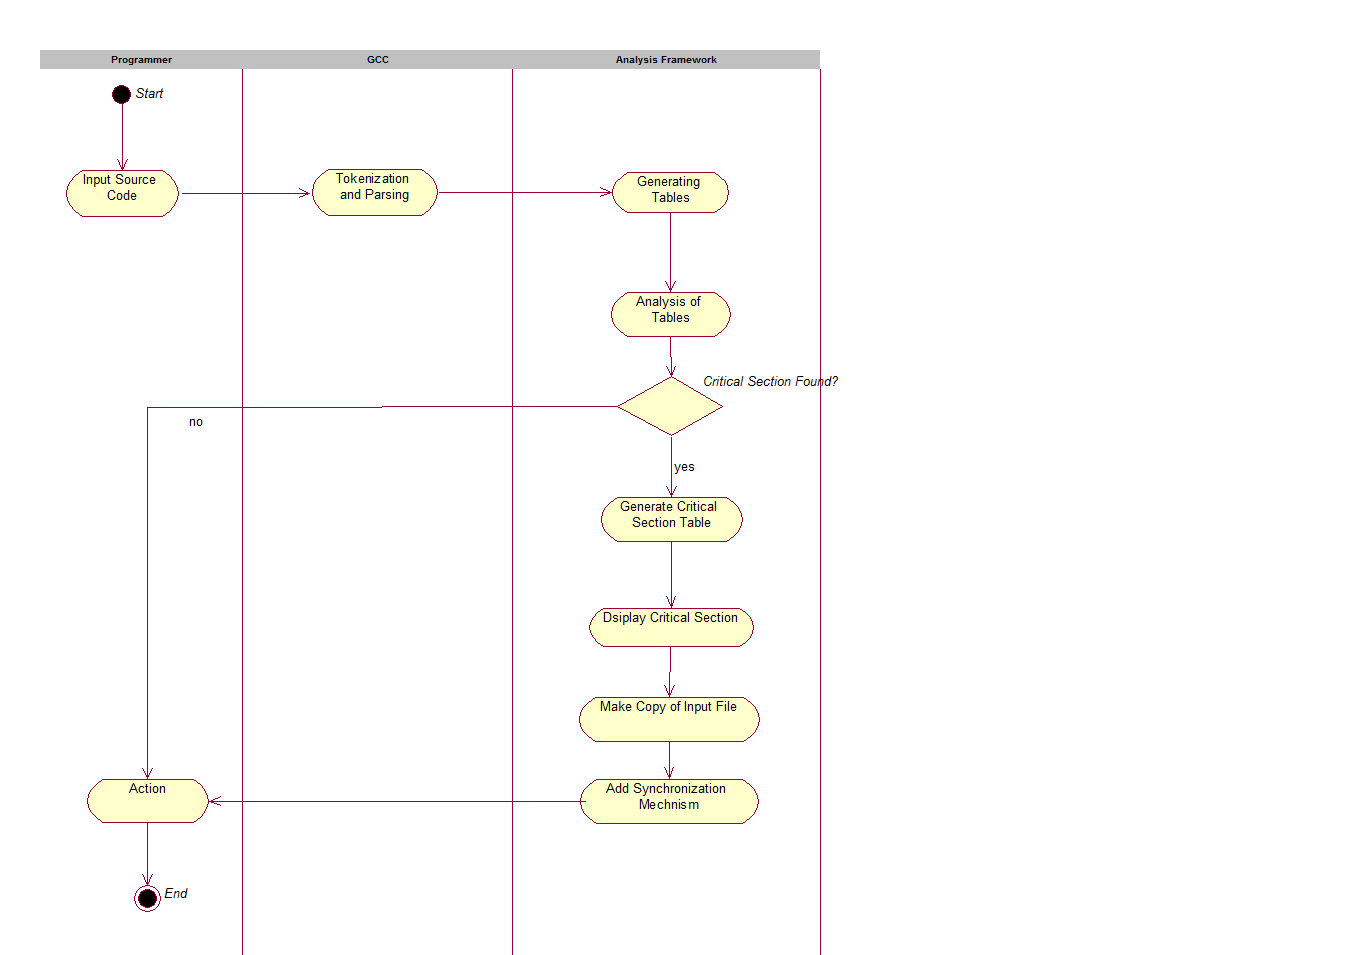
\includegraphics[scale=0.6]{activity.png}
\caption{Activity Diagram}
\label{<<Label>>}
\end{figure}
\paragraph{}
From programmers prespective activity diagram shows which are the diffrent activities performed by Programmer, GCC and the Analysis Framework.

\subsection{Component Diagram}
\begin{figure}[H]
\centering
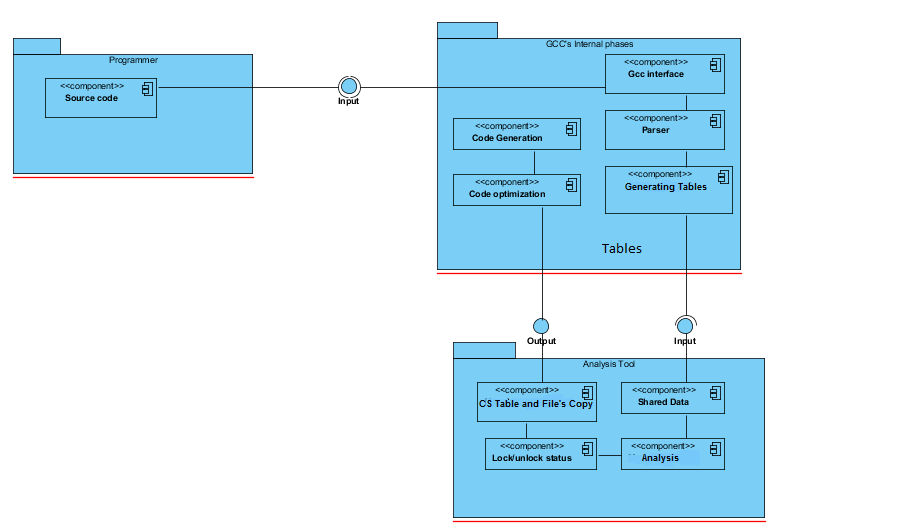
\includegraphics[scale=0.6]{component.png}
\caption{Component Diagram}
\label{<<Label>>}
\end{figure}
\paragraph{}
From Component point of view our system having different components used in system like system is Table Generator which generates the tables like Global Symbol's Table, Local Symbol's Table, Log Table, Semaphore Table, Function Table and Thread Table etc.

\subsection{Deployment Diagram}
\begin{figure}[H]
\centering
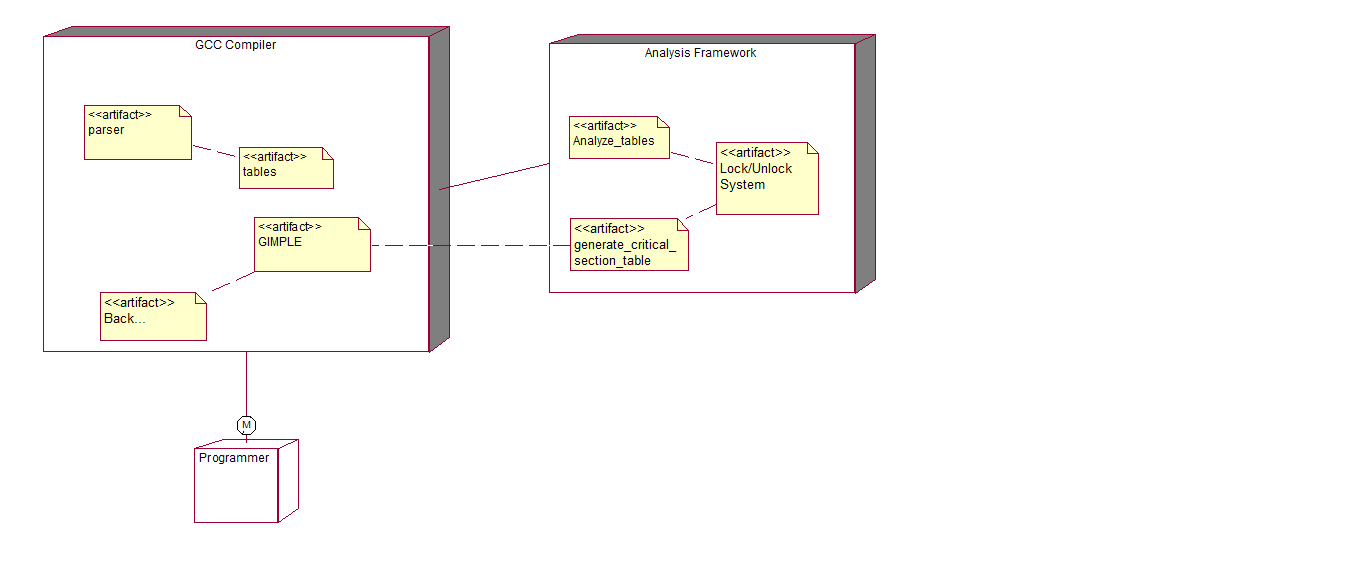
\includegraphics[scale=0.6]{deployment.png}
\caption{Deployment Diagram}
\label{<<Label>>}
\end{figure}
\paragraph{}
From deployment point of view our system contains following hardware and software component which are required for system execution are like GCC Compiler for compiling the source code, lex and yacc for Tokenization and Parsiing and the analysis frmaework for detecting the critical sections and adding synchronization mechanism.
